% Options for packages loaded elsewhere
\PassOptionsToPackage{unicode}{hyperref}
\PassOptionsToPackage{hyphens}{url}
\PassOptionsToPackage{dvipsnames,svgnames,x11names}{xcolor}
%
\documentclass[
  letterpaper,
  DIV=11,
  numbers=noendperiod]{scrartcl}

\usepackage{amsmath,amssymb}
\usepackage{iftex}
\ifPDFTeX
  \usepackage[T1]{fontenc}
  \usepackage[utf8]{inputenc}
  \usepackage{textcomp} % provide euro and other symbols
\else % if luatex or xetex
  \usepackage{unicode-math}
  \defaultfontfeatures{Scale=MatchLowercase}
  \defaultfontfeatures[\rmfamily]{Ligatures=TeX,Scale=1}
\fi
\usepackage{lmodern}
\ifPDFTeX\else  
    % xetex/luatex font selection
\fi
% Use upquote if available, for straight quotes in verbatim environments
\IfFileExists{upquote.sty}{\usepackage{upquote}}{}
\IfFileExists{microtype.sty}{% use microtype if available
  \usepackage[]{microtype}
  \UseMicrotypeSet[protrusion]{basicmath} % disable protrusion for tt fonts
}{}
\makeatletter
\@ifundefined{KOMAClassName}{% if non-KOMA class
  \IfFileExists{parskip.sty}{%
    \usepackage{parskip}
  }{% else
    \setlength{\parindent}{0pt}
    \setlength{\parskip}{6pt plus 2pt minus 1pt}}
}{% if KOMA class
  \KOMAoptions{parskip=half}}
\makeatother
\usepackage{xcolor}
\setlength{\emergencystretch}{3em} % prevent overfull lines
\setcounter{secnumdepth}{-\maxdimen} % remove section numbering
% Make \paragraph and \subparagraph free-standing
\makeatletter
\ifx\paragraph\undefined\else
  \let\oldparagraph\paragraph
  \renewcommand{\paragraph}{
    \@ifstar
      \xxxParagraphStar
      \xxxParagraphNoStar
  }
  \newcommand{\xxxParagraphStar}[1]{\oldparagraph*{#1}\mbox{}}
  \newcommand{\xxxParagraphNoStar}[1]{\oldparagraph{#1}\mbox{}}
\fi
\ifx\subparagraph\undefined\else
  \let\oldsubparagraph\subparagraph
  \renewcommand{\subparagraph}{
    \@ifstar
      \xxxSubParagraphStar
      \xxxSubParagraphNoStar
  }
  \newcommand{\xxxSubParagraphStar}[1]{\oldsubparagraph*{#1}\mbox{}}
  \newcommand{\xxxSubParagraphNoStar}[1]{\oldsubparagraph{#1}\mbox{}}
\fi
\makeatother

\usepackage{color}
\usepackage{fancyvrb}
\newcommand{\VerbBar}{|}
\newcommand{\VERB}{\Verb[commandchars=\\\{\}]}
\DefineVerbatimEnvironment{Highlighting}{Verbatim}{commandchars=\\\{\}}
% Add ',fontsize=\small' for more characters per line
\usepackage{framed}
\definecolor{shadecolor}{RGB}{241,243,245}
\newenvironment{Shaded}{\begin{snugshade}}{\end{snugshade}}
\newcommand{\AlertTok}[1]{\textcolor[rgb]{0.68,0.00,0.00}{#1}}
\newcommand{\AnnotationTok}[1]{\textcolor[rgb]{0.37,0.37,0.37}{#1}}
\newcommand{\AttributeTok}[1]{\textcolor[rgb]{0.40,0.45,0.13}{#1}}
\newcommand{\BaseNTok}[1]{\textcolor[rgb]{0.68,0.00,0.00}{#1}}
\newcommand{\BuiltInTok}[1]{\textcolor[rgb]{0.00,0.23,0.31}{#1}}
\newcommand{\CharTok}[1]{\textcolor[rgb]{0.13,0.47,0.30}{#1}}
\newcommand{\CommentTok}[1]{\textcolor[rgb]{0.37,0.37,0.37}{#1}}
\newcommand{\CommentVarTok}[1]{\textcolor[rgb]{0.37,0.37,0.37}{\textit{#1}}}
\newcommand{\ConstantTok}[1]{\textcolor[rgb]{0.56,0.35,0.01}{#1}}
\newcommand{\ControlFlowTok}[1]{\textcolor[rgb]{0.00,0.23,0.31}{\textbf{#1}}}
\newcommand{\DataTypeTok}[1]{\textcolor[rgb]{0.68,0.00,0.00}{#1}}
\newcommand{\DecValTok}[1]{\textcolor[rgb]{0.68,0.00,0.00}{#1}}
\newcommand{\DocumentationTok}[1]{\textcolor[rgb]{0.37,0.37,0.37}{\textit{#1}}}
\newcommand{\ErrorTok}[1]{\textcolor[rgb]{0.68,0.00,0.00}{#1}}
\newcommand{\ExtensionTok}[1]{\textcolor[rgb]{0.00,0.23,0.31}{#1}}
\newcommand{\FloatTok}[1]{\textcolor[rgb]{0.68,0.00,0.00}{#1}}
\newcommand{\FunctionTok}[1]{\textcolor[rgb]{0.28,0.35,0.67}{#1}}
\newcommand{\ImportTok}[1]{\textcolor[rgb]{0.00,0.46,0.62}{#1}}
\newcommand{\InformationTok}[1]{\textcolor[rgb]{0.37,0.37,0.37}{#1}}
\newcommand{\KeywordTok}[1]{\textcolor[rgb]{0.00,0.23,0.31}{\textbf{#1}}}
\newcommand{\NormalTok}[1]{\textcolor[rgb]{0.00,0.23,0.31}{#1}}
\newcommand{\OperatorTok}[1]{\textcolor[rgb]{0.37,0.37,0.37}{#1}}
\newcommand{\OtherTok}[1]{\textcolor[rgb]{0.00,0.23,0.31}{#1}}
\newcommand{\PreprocessorTok}[1]{\textcolor[rgb]{0.68,0.00,0.00}{#1}}
\newcommand{\RegionMarkerTok}[1]{\textcolor[rgb]{0.00,0.23,0.31}{#1}}
\newcommand{\SpecialCharTok}[1]{\textcolor[rgb]{0.37,0.37,0.37}{#1}}
\newcommand{\SpecialStringTok}[1]{\textcolor[rgb]{0.13,0.47,0.30}{#1}}
\newcommand{\StringTok}[1]{\textcolor[rgb]{0.13,0.47,0.30}{#1}}
\newcommand{\VariableTok}[1]{\textcolor[rgb]{0.07,0.07,0.07}{#1}}
\newcommand{\VerbatimStringTok}[1]{\textcolor[rgb]{0.13,0.47,0.30}{#1}}
\newcommand{\WarningTok}[1]{\textcolor[rgb]{0.37,0.37,0.37}{\textit{#1}}}

\providecommand{\tightlist}{%
  \setlength{\itemsep}{0pt}\setlength{\parskip}{0pt}}\usepackage{longtable,booktabs,array}
\usepackage{calc} % for calculating minipage widths
% Correct order of tables after \paragraph or \subparagraph
\usepackage{etoolbox}
\makeatletter
\patchcmd\longtable{\par}{\if@noskipsec\mbox{}\fi\par}{}{}
\makeatother
% Allow footnotes in longtable head/foot
\IfFileExists{footnotehyper.sty}{\usepackage{footnotehyper}}{\usepackage{footnote}}
\makesavenoteenv{longtable}
\usepackage{graphicx}
\makeatletter
\newsavebox\pandoc@box
\newcommand*\pandocbounded[1]{% scales image to fit in text height/width
  \sbox\pandoc@box{#1}%
  \Gscale@div\@tempa{\textheight}{\dimexpr\ht\pandoc@box+\dp\pandoc@box\relax}%
  \Gscale@div\@tempb{\linewidth}{\wd\pandoc@box}%
  \ifdim\@tempb\p@<\@tempa\p@\let\@tempa\@tempb\fi% select the smaller of both
  \ifdim\@tempa\p@<\p@\scalebox{\@tempa}{\usebox\pandoc@box}%
  \else\usebox{\pandoc@box}%
  \fi%
}
% Set default figure placement to htbp
\def\fps@figure{htbp}
\makeatother

\KOMAoption{captions}{tableheading}
\makeatletter
\@ifpackageloaded{caption}{}{\usepackage{caption}}
\AtBeginDocument{%
\ifdefined\contentsname
  \renewcommand*\contentsname{Table of contents}
\else
  \newcommand\contentsname{Table of contents}
\fi
\ifdefined\listfigurename
  \renewcommand*\listfigurename{List of Figures}
\else
  \newcommand\listfigurename{List of Figures}
\fi
\ifdefined\listtablename
  \renewcommand*\listtablename{List of Tables}
\else
  \newcommand\listtablename{List of Tables}
\fi
\ifdefined\figurename
  \renewcommand*\figurename{Figure}
\else
  \newcommand\figurename{Figure}
\fi
\ifdefined\tablename
  \renewcommand*\tablename{Table}
\else
  \newcommand\tablename{Table}
\fi
}
\@ifpackageloaded{float}{}{\usepackage{float}}
\floatstyle{ruled}
\@ifundefined{c@chapter}{\newfloat{codelisting}{h}{lop}}{\newfloat{codelisting}{h}{lop}[chapter]}
\floatname{codelisting}{Listing}
\newcommand*\listoflistings{\listof{codelisting}{List of Listings}}
\makeatother
\makeatletter
\makeatother
\makeatletter
\@ifpackageloaded{caption}{}{\usepackage{caption}}
\@ifpackageloaded{subcaption}{}{\usepackage{subcaption}}
\makeatother

\usepackage{bookmark}

\IfFileExists{xurl.sty}{\usepackage{xurl}}{} % add URL line breaks if available
\urlstyle{same} % disable monospaced font for URLs
\hypersetup{
  pdftitle={Modelo de regressão logística e Modelos de risco proporcionais (Cox)},
  colorlinks=true,
  linkcolor={blue},
  filecolor={Maroon},
  citecolor={Blue},
  urlcolor={Blue},
  pdfcreator={LaTeX via pandoc}}


\title{Modelo de regressão logística e Modelos de risco proporcionais
(Cox)}
\author{}
\date{}

\begin{document}
\maketitle


\section{Modelos prognósticos}\label{modelos-prognuxf3sticos}

\subsection{Modelos prognósticos}\label{modelos-prognuxf3sticos-1}

\textbf{Prognóstico} significa prever, predizer ou estimar a
probabilidade ou risco de \textbf{condições futuras}.

. . .

Na área da saúde, prognóstico comumente relaciona-se à probabilidade ou
risco de um \textbf{indivíduo} desenvolver um particular estado de saúde
(um desfecho) ao longo de um período de tempo específico, baseado na
presença ou ausência de um perfil clínico.

. . .

\textbf{Regressão linear}, \textbf{logística} e \textbf{de risco}
(análise de sobrevida) são métodos comuns utilizados na pesquisa clínica
para relatar covariáveis e desfechos.

\subsection{Modelos prognósticos}\label{modelos-prognuxf3sticos-2}

A \textbf{regressão linear} é o método padrão para \textbf{desfechos
contínuos}.

. . .

A \textbf{regressão logística} é adequada para \textbf{desfechos
binários}

. . .

Quando desfechos binários são medidos \textbf{prospectivamente}, eles
também são associados com um tempo para o evento. Neste caso, a
\textbf{regressão logística} ou a \textbf{análise de sobrevida} podem
ser adequadas.

\subsection{Modelos de regressão
linear}\label{modelos-de-regressuxe3o-linear}

Na regressão linear, ajustamos um modelo do tipo

\[Y = \beta_0 + \beta_1X_1+ \dots + \beta_iX_i + \varepsilon\]

. . .

\begin{itemize}
\tightlist
\item
  \textbf{Pressuposto importante:} a variável \(Y\) era de natureza
  \textbf{contínua} e seguia uma distribuição normal.
\end{itemize}

. . .

O modelo se preocupava em estimar (ou predizer) o valor médio de \(Y\)
dado um certo conjunto de valores das variáveis explicativas.

\subsection{Modelos de regressão
linear}\label{modelos-de-regressuxe3o-linear-1}

Em um modelo de regressão linear, as variáveis explicativas podem ser
\textbf{contínuas} ou \textbf{dicotômicas}.

. . .

O \textbf{coeficiente} para uma covariável contínua depende, em grande
parte, das unidades, e a \textbf{magnitude} só pode ser interpretada em
um \textbf{contexto clínico}.

. . .

Se um pesquisador quer saber a \textbf{mudança esperada na resposta}
para um aumento de 10 unidades (ou qualquer outro aumento) em uma
covariável contínua, ele pode simplesmente multiplicar o coeficiente (e
os limites de confiança) por 10.

. . .

Para covariáveis \textbf{dicotômicas}, o coeficiente é interpretado como
a \textbf{diferença na resposta} que seria vista, em média, entre os
dois níveis da covariável.

\section{Exemplo}\label{exemplo}

\subsection{Descrição da base de
dados}\label{descriuxe7uxe3o-da-base-de-dados}

O \href{https://www.cdc.gov/nchs/nhanes/index.html}{NHANES} (National
Health and Nutrition Examination Survey) é um estudo populacional dos
EUA que contém dados de saúde.

. . .

Vamos estimar um modelo de regressão linear múltiplo usando os dados do
NHANES, incluindo covariáveis clínicas e demográficas.

\subsection{Descrição da base de
dados}\label{descriuxe7uxe3o-da-base-de-dados-1}

Usaremos a pressão arterial sistólica (PAS) como variável dependente e
as seguintes variáveis independentes:

\begin{itemize}
\tightlist
\item
  IMC (quanto maior o IMC, maior pode ser a pressão arterial?)
\item
  Idade (o envelhecimento está associado ao aumento da PAS?)
\item
  Sexo (homens têm maior PAS que mulheres?)
\item
  Horas de sono à noite (SleepHrsNight) (dormir mais pode diminuir a
  PAS?)
\item
  Nível de colesterol total (TotChol) (colesterol elevado está associado
  a maior PAS?)
\item
  Tabagismo (SmokeNow) (fumantes têm PAS mais alta?)
\end{itemize}

\subsection{Preparação}\label{preparauxe7uxe3o}

\subsubsection{Carregando os pacotes R}\label{carregando-os-pacotes-r}

\begin{Shaded}
\begin{Highlighting}[]
\NormalTok{pacman}\SpecialCharTok{::}\FunctionTok{p\_load}\NormalTok{(}
\NormalTok{NHANES,}
\NormalTok{tidyverse,}
\NormalTok{car,}
\NormalTok{lmtest,}
\NormalTok{mfx}
\NormalTok{  ) }
\end{Highlighting}
\end{Shaded}

\subsection{Carregando os dados}\label{carregando-os-dados}

\begin{Shaded}
\begin{Highlighting}[]
\CommentTok{\# Selecionar variáveis relevantes e remover NAs}
\NormalTok{dados }\OtherTok{\textless{}{-}}\NormalTok{ NHANES }\SpecialCharTok{\%\textgreater{}\%}
  \FunctionTok{filter}\NormalTok{(}\SpecialCharTok{!}\FunctionTok{is.na}\NormalTok{(BPSysAve) }\SpecialCharTok{\&} \SpecialCharTok{!}\FunctionTok{is.na}\NormalTok{(BMI) }\SpecialCharTok{\&} \SpecialCharTok{!}\FunctionTok{is.na}\NormalTok{(Age) }\SpecialCharTok{\&} \SpecialCharTok{!}\FunctionTok{is.na}\NormalTok{(Gender) }\SpecialCharTok{\&} 
           \SpecialCharTok{!}\FunctionTok{is.na}\NormalTok{(TotChol) }\SpecialCharTok{\&} \SpecialCharTok{!}\FunctionTok{is.na}\NormalTok{(SleepHrsNight) }\SpecialCharTok{\&} \SpecialCharTok{!}\FunctionTok{is.na}\NormalTok{(SmokeNow)) }\SpecialCharTok{\%\textgreater{}\%}
\NormalTok{  dplyr}\SpecialCharTok{::}\FunctionTok{select}\NormalTok{(BPSysAve, BMI, Age, Gender, TotChol,SleepHrsNight,  SmokeNow)}
\end{Highlighting}
\end{Shaded}

\subsection{Manipulação dos dados}\label{manipulauxe7uxe3o-dos-dados}

\begin{Shaded}
\begin{Highlighting}[]
\CommentTok{\# Renomear variáveis para facilitar}
\FunctionTok{colnames}\NormalTok{(dados) }\OtherTok{\textless{}{-}} \FunctionTok{c}\NormalTok{(}\StringTok{"PAS"}\NormalTok{, }\StringTok{"IMC"}\NormalTok{, }\StringTok{"Idade"}\NormalTok{, }\StringTok{"Sexo"}\NormalTok{, }\StringTok{"Colesterol"}\NormalTok{, }\StringTok{"HorasDeSonoNoite"}\NormalTok{, }\StringTok{"Fumante"}\NormalTok{)}

\CommentTok{\# Transformar Sexo e Fumante em fatores}
\NormalTok{dados}\SpecialCharTok{$}\NormalTok{Sexo }\OtherTok{\textless{}{-}} \FunctionTok{as.factor}\NormalTok{(dados}\SpecialCharTok{$}\NormalTok{Sexo)}
\NormalTok{dados}\SpecialCharTok{$}\NormalTok{Fumante }\OtherTok{\textless{}{-}} \FunctionTok{as.factor}\NormalTok{(dados}\SpecialCharTok{$}\NormalTok{Fumante)}

\CommentTok{\# Estrutura dos dados}

\NormalTok{dados }\SpecialCharTok{\%\textgreater{}\%} 
  \FunctionTok{str}\NormalTok{()}
\end{Highlighting}
\end{Shaded}

\begin{verbatim}
tibble [2,940 x 7] (S3: tbl_df/tbl/data.frame)
 $ PAS             : int [1:2940] 113 113 113 112 111 127 128 152 122 144 ...
 $ IMC             : num [1:2940] 32.2 32.2 32.2 30.6 23.7 ...
 $ Idade           : int [1:2940] 34 34 34 49 66 58 33 60 57 44 ...
 $ Sexo            : Factor w/ 2 levels "female","male": 2 2 2 1 2 1 2 2 1 2 ...
 $ Colesterol      : num [1:2940] 3.49 3.49 3.49 6.7 4.99 4.78 5.59 6.39 5.04 5.61 ...
 $ HorasDeSonoNoite: int [1:2940] 4 4 4 8 7 5 6 6 8 4 ...
 $ Fumante         : Factor w/ 2 levels "No","Yes": 1 1 1 2 1 2 1 1 1 2 ...
\end{verbatim}

\subsection{Ajuste do modelo}\label{ajuste-do-modelo}

\begin{Shaded}
\begin{Highlighting}[]
\CommentTok{\# Ajustar modelo de regressão linear múltiplo}
\NormalTok{modelo\_multiplo }\OtherTok{\textless{}{-}} \FunctionTok{lm}\NormalTok{(PAS }\SpecialCharTok{\textasciitilde{}}\NormalTok{ IMC }\SpecialCharTok{+}\NormalTok{ Idade }\SpecialCharTok{+}\NormalTok{ Sexo }\SpecialCharTok{+}\NormalTok{ Colesterol }\SpecialCharTok{+}\NormalTok{ HorasDeSonoNoite }\SpecialCharTok{+}\NormalTok{ Fumante, }\AttributeTok{data =}\NormalTok{ dados)}

\CommentTok{\# Resumo do modelo}
\FunctionTok{summary}\NormalTok{(modelo\_multiplo)}
\end{Highlighting}
\end{Shaded}

\begin{verbatim}

Call:
lm(formula = PAS ~ IMC + Idade + Sexo + Colesterol + HorasDeSonoNoite + 
    Fumante, data = dados)

Residuals:
    Min      1Q  Median      3Q     Max 
-56.440  -9.003  -1.070   8.170  83.997 

Coefficients:
                 Estimate Std. Error t value Pr(>|t|)    
(Intercept)      88.82356    2.63293  33.736  < 2e-16 ***
IMC               0.17376    0.04634   3.750 0.000181 ***
Idade             0.42727    0.01868  22.876  < 2e-16 ***
Sexomale          4.91074    0.59226   8.292  < 2e-16 ***
Colesterol        1.46760    0.27216   5.392  7.5e-08 ***
HorasDeSonoNoite -0.42090    0.21150  -1.990 0.046674 *  
FumanteYes        0.63493    0.62894   1.010 0.312811    
---
Signif. codes:  0 '***' 0.001 '**' 0.01 '*' 0.05 '.' 0.1 ' ' 1

Residual standard error: 15.86 on 2933 degrees of freedom
Multiple R-squared:  0.1956,    Adjusted R-squared:  0.194 
F-statistic: 118.9 on 6 and 2933 DF,  p-value: < 2.2e-16
\end{verbatim}

\subsection{Interpretação do
modelo}\label{interpretauxe7uxe3o-do-modelo}

\begin{longtable}[]{@{}cccc@{}}
\toprule\noalign{}
& & & \\
Variável & Coeficiente (β) & p-valor & Interpretação \\
\midrule\noalign{}
\endhead
\bottomrule\noalign{}
\endlastfoot
Intercepto & 88,82 & \textless{} 0,001 & Valor médio da PAS quando todas
as variáveis preditoras são zero. \\
IMC & 0,17 & \textless{} 0,001 & A cada aumento de 1 unidade no IMC, a
PAS aumenta, em média, 0,17 mmHg, ajustado para as demais variáveis. \\
Idade & 0,42 & \textless{} 0,001 & A cada ano a mais de idade, a PAS
aumenta 0.42 mmHg. \\
Sexo (Masculino) & 4,91 & \textless{} 0,001 & O sexo masculino foi
associado a uma PAS 4,91 mmHg maior que no sexo feminino, em média. \\
Colesterol & 1,47 & \textless{} 0,001 & Para cada aumento de 1 mg/dL no
colesterol, a PAS aumenta 1,47 mmHg. \\
Horas de sono & -0,42 & 0,047 & Para cada aumento de 1 h dormida a
noite, a PAS diminui 0,42 mmHg. \\
Fumante (Sim) & 0,64 & 0,312 & Não significativo (p \textgreater{}
0.05), indicando que o tabagismo não teve efeito estatisticamente
relevante na PAS. \\
& & & \\
\end{longtable}

\subsection{Variável dependente (desfecho)
binária}\label{variuxe1vel-dependente-desfecho-binuxe1ria}

E se a variável dependente \(y\) for \textbf{binária}?

\begin{itemize}
\tightlist
\item
  Doença (presente = 1/ausente = 0)
\item
  Morto = 1/Vivo = 0
\end{itemize}

. . .

Aqui, \(Y = 1\) corresponde ao sucesso, ou seja, a ocorrência do evento
e \(Y = 0\) corresponde ao fracasso, ou seja, à não ocorrência do
evento.

. . .

Temos então que a média de \(Y\) é igual a \(p\), sendo \(p\) a
proporção de vezes que \(Y\) assume o valor 1. Assim,

\[p = P(Y=1) = P(\text{sucesso})\]

\subsection{Variável dependente (desfecho)
binária}\label{variuxe1vel-dependente-desfecho-binuxe1ria-1}

A regressão logística é um modelo estatístico que permite estimar a
probabilidade \(p\) da ocorrência de um determinado desfecho categórico
(Y) em função de um ou mais preditores (X), que podem ser contínuos ou
categóricos.

. . .

Vamos a um exemplo\ldots{}

\subsection{Variável dependente (desfecho)
binária}\label{variuxe1vel-dependente-desfecho-binuxe1ria-2}

Considere a população de bebês com baixo peso ao nascer (definido como
\textless{} 1750g) que estão confinados em uma unidade de tratamento
intensivo neonatal, entubados durante as primeiras 12 semanas de vida e
sobreviventes por, no mínimo, 28 dias.

Na amostra de 223 bebês extraída da população original, 76 foram
diagnosticados com \emph{displasia broncopulmonar} (BPD). Os restantes
147 não tinham a doença.

Seja \(Y\) uma variável aleatória dicotômica, de forma que

\[Y = \begin{cases} 0 & \text{Ausência de BPD} \\ 1 & \text{Presença de BPD} \end{cases}\]

\subsection{Variável dependente (desfecho)
binária}\label{variuxe1vel-dependente-desfecho-binuxe1ria-3}

A probabilidade estimada de que um bebê dessa população desenvolva BPD é
a \textbf{proporção amostral} de bebês com BPD, ou seja,

\[\hat{p} = \dfrac{76}{223} = 0,341\]

. . .

Podemos suspeitar que alguns fatores, maternos ou neonatais, devem
afetar a probabilidade de um bebê em particular desenvolver BPD.

. . .

O conhecimento da presença ou ausência desses fatores pode:

\begin{itemize}
\item
  aumentar a precisão de nossa estimativa de \(p\),
\item
  desenvolverintervenções para reduzir essa probabilidade.
\end{itemize}

\subsection{Variável dependente (desfecho)
binária}\label{variuxe1vel-dependente-desfecho-binuxe1ria-4}

\begin{itemize}
\tightlist
\item
  Um fator interessante poderia ser o peso de nascimento de um bebê, que
  chamaremos de \(X\).
\end{itemize}

. . .

\begin{itemize}
\tightlist
\item
  Se a variável \(Y\) fosse \textbf{contínua}, poderíamos começar a
  análise contruindo um diagrama de dispersão entre as variáveis \(X\) e
  \(Y\).
\end{itemize}

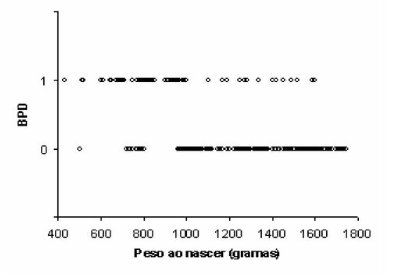
\includegraphics[width=6.25in,height=4.6875in]{../../images/BPD_disp.png}

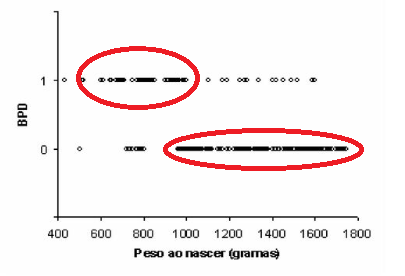
\includegraphics[width=6.25in,height=4.6875in]{../../images/BPD_disp2.png}

\begin{longtable}[]{@{}
  >{\centering\arraybackslash}p{(\linewidth - 6\tabcolsep) * \real{0.2500}}
  >{\centering\arraybackslash}p{(\linewidth - 6\tabcolsep) * \real{0.2500}}
  >{\centering\arraybackslash}p{(\linewidth - 6\tabcolsep) * \real{0.2500}}
  >{\centering\arraybackslash}p{(\linewidth - 6\tabcolsep) * \real{0.2500}}@{}}
\toprule\noalign{}
\begin{minipage}[b]{\linewidth}\centering
\end{minipage} & \begin{minipage}[b]{\linewidth}\centering
\end{minipage} & \begin{minipage}[b]{\linewidth}\centering
\end{minipage} & \begin{minipage}[b]{\linewidth}\centering
\end{minipage} \\
\begin{minipage}[b]{\linewidth}\centering
Peso(g)
\end{minipage} & \begin{minipage}[b]{\linewidth}\centering
n
\end{minipage} & \begin{minipage}[b]{\linewidth}\centering
BPD
\end{minipage} & \begin{minipage}[b]{\linewidth}\centering
p
\end{minipage} \\
\midrule\noalign{}
\endhead
\bottomrule\noalign{}
\endlastfoot
0-950 & 68 & 49 & 0,721 \\
951-1350 & 80 & 18 & 0,225 \\
1351-1750 & 75 & 9 & 0,120 \\
& 223 & 76 & 0,341 \\
\begin{minipage}[t]{\linewidth}\centering
\end{minipage} & & & \\
\end{longtable}

\subsection{Variável dependente (desfecho)
binária}\label{variuxe1vel-dependente-desfecho-binuxe1ria-5}

\begin{itemize}
\tightlist
\item
  Parece que a probabilidade de desenvolver BPD aumenta à medida que o
  peso do bebê ao nascer diminui e vice-versa.
\end{itemize}

. . .

\begin{itemize}
\tightlist
\item
  Como parece haver uma relação entre estas duas variáveis, podemos usar
  o peso ao nascer de uma criança para nos ajudar a prever a
  probabilidade de que ela desenvolva BPD.
\end{itemize}

\subsection{Função logística}\label{funuxe7uxe3o-loguxedstica}

A primeira estratégia poderia ser ajustar um modelo da forma

\[p = \beta_0 + \beta_1 x\] onde \(x\) representa o peso ao nascer.

. . .

Sob inspeção, este modelo não é viável, uma vez que \(p\) é uma
probabilidade, podendo assumir, portanto, valores entre 0 e 1.

. . .

O termo \(\beta_0 + \beta_1 x\), ao contrário, pode assumir valores fora
desse intervalo.

\subsection{Função logística}\label{funuxe7uxe3o-loguxedstica-1}

Uma alternativa seria ajustar o modelo

\[p = e^{\beta_0 + \beta_1 x}\]

Essa expressão garante que a estimativa de \(p\) é sempre positiva.

. . .

No entanto, este modelo também é inadequado, uma vez que pode produzir
valores maiores que 1.

\subsection{Função logística}\label{funuxe7uxe3o-loguxedstica-2}

Podemos então, ajustar um modelo da forma

\[p = \dfrac{e^{\beta_0 + \beta_1 x}}{1 + e^{\beta_0 + \beta_1 x}}\]

. . .

Esta expressão, conhecida como \textbf{função logística}, não admite
valores negativos nem maiores que 1.

\subsection{Função logística}\label{funuxe7uxe3o-loguxedstica-3}

Lembre-se de que, se um evento ocorre com probabilidade \(p\), a
\textbf{chance} a seu favor é de \(\dfrac{p}{1-p}\) para 1.

. . .

Assim, se um \textbf{sucesso} ocorre com probabilidade

\[p = \dfrac{e^{\beta_0 + \beta_1 x}}{1 + e^{\beta_0 + \beta_1 x}},\]

\subsection{Função logística}\label{funuxe7uxe3o-loguxedstica-4}

a \textbf{chance} em favor de sucesso é

\[\dfrac{p}{1-p} = \dfrac{\dfrac{e^{\beta_0 + \beta_1 x}}{1 + e^{\beta_0 + \beta_1 x}}}{\dfrac{1}{1 + e^{\beta_0 + \beta_1 x}}} = e^{\beta_0 + \beta_1 x}\]

. . .

Tomando o logaritmo natural de cada lado dessa equação,

\[\underbrace{\ln\left ( \frac{p}{1-p} \right)}_\text{logit} = \ln(e^{\beta_0 + \beta_1 x}) = \beta_0 + \beta_1 x\]

\subsection{Modelo de regressão
logística}\label{modelo-de-regressuxe3o-loguxedstica}

Modelar uma probabilidade \(p\) com uma função logística é
\textbf{equivalente} a ajustar um modelo de regressão linear onde a
variável dependente contínua \(y\) foi substituída pelo logaritmo
neperiano da \textbf{chance} de ocorrência de um evento
\textbf{dicotômico}.

. . .

Em vez de assumir que a relação entre \(p\) e \(X\) é \textbf{linear},
assume-se que a relação entre \(\ln\left ( \frac{p}{1-p} \right)\) e
\(X\) é \textbf{linear}.

. . .

Essa técnica é conhecida como \textbf{regressão logística}.

\subsection{Modelo de regressão
logística}\label{modelo-de-regressuxe3o-loguxedstica-1}

Os parâmetros do modelo (\(\beta\)'s) são estimados usando o
\textbf{método de máxima verossimilhança}, que busca maximizar a
probabilidade de observar os dados dados os parâmetros.

. . .

Este processo envolve iterativamente ajustar os coeficientes para melhor
se alinhar com os dados observados.

\[\ln\left ( \frac{\hat{p}}{1-\hat{p}} \right) = \hat{\beta}_0 + \hat{\beta}_1 x\]

\subsection{Modelo de regressão
logística}\label{modelo-de-regressuxe3o-loguxedstica-2}

Voltando ao exemplo, para a amostra de 223 bebês com baixo peso ao
nascer, a equação da regressão logística estimada é

\[\ln\left ( \frac{\hat{p}}{1-\hat{p}} \right) = 4,0343 - 0,0042 x\]

. . .

\begin{itemize}
\tightlist
\item
  \textbf{Interpretação:} O coeficiente do peso indica que, para cada
  aumento de 1 grama no peso ao nascer, o logaritmo da chance de que um
  bebê desenvolva BPD diminui de 0,0042, em média.
\end{itemize}

\subsection{Modelo de regressão
logística}\label{modelo-de-regressuxe3o-loguxedstica-3}

Qual a probabilidade de que um bebê, retirado desta população pesando
750g ao nascer, irá desenvolver BPD?

\[
\begin{eqnarray*}
\ln\left ( \frac{\hat{p}}{1-\hat{p}} \right) = 4,0343 - 0,0042 x
\end{eqnarray*}
\]

. . .

Trocando-se \(x\) por 750, temos

\[
\begin{eqnarray*}
\ln\left ( \frac{\hat{p}}{1-\hat{p}} \right) = 4,0343 - 0,0042 \times 750 = 0,8843
\end{eqnarray*}
\]

\subsection{Modelo de regressão
logística}\label{modelo-de-regressuxe3o-loguxedstica-4}

Aplicando a função exponencial em ambos os lados, temos

\[
\begin{eqnarray*}
\ln\left ( \frac{\hat{p}}{1-\hat{p}} \right) &=& 0,8843 \\ \frac{\hat{p}}{1-\hat{p}} &=& e^{0,8843} = 2,4113
\end{eqnarray*}
\]

\subsection{Modelo de regressão
logística}\label{modelo-de-regressuxe3o-loguxedstica-5}

Isolando \(\hat{p}\):

\[
\begin{eqnarray*}
\frac{\hat{p}}{1-\hat{p}} &=& 2,4113 \\ \hat{p} &=& 2,4113 - 2,4113 \hat{p} \\ \hat{p} + 2,4113 \hat{p} &=& 2,4113 \\ (1 + 2,4113)\hat{p} &=& 2,4113 \\ \hat{p} &=& \dfrac{2,4113}{1 + 2,4113} = 0,708
\end{eqnarray*}
\]

\subsection{Modelo de regressão
logística}\label{modelo-de-regressuxe3o-loguxedstica-6}

A probabilidade estimada de que uma criança, que pesa 750g ao nascer,
desenvolva BPD é de 0,708.

. . .

Se calculássemos a probabilidade estimada \(\hat{p}\) para cada valor
observado dos pesos ao nascer e plotássemos \(\hat{p} \times\) o peso,
teríamos

\begin{center}
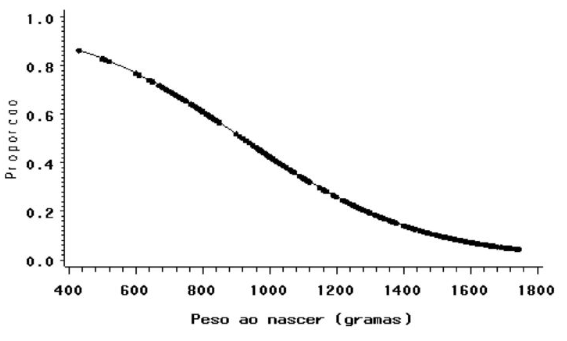
\includegraphics[width=6.25in,height=4.6875in]{../../images/graf_logs.png}
\end{center}

\section{Exemplo}\label{exemplo-1}

\subsection{Descrição da base de
dados}\label{descriuxe7uxe3o-da-base-de-dados-2}

O \href{https://www.cdc.gov/nchs/nhanes/index.html}{NHANES} (National
Health and Nutrition Examination Survey) é um estudo populacional dos
EUA que contém dados de saúde.

. . .

Vamos estimar um modelo de regressão logística usando os dados do
NHANES, incluindo covariáveis clínicas e demográficas.

\subsection{Descrição da base de
dados}\label{descriuxe7uxe3o-da-base-de-dados-3}

Usaremos \emph{Diabetes} como variável dependente e as seguintes
variáveis independentes:

\begin{itemize}
\tightlist
\item
  PAS (a pressão arterial sistólica está associada à diabetes?)
\item
  IMC (IMC está associado à diabetes?)
\item
  Idade (o envelhecimento está associado à diabetes?)
\item
  Sexo (homens têm maior risco de ter diabetes que mulheres?)
\item
  Horas de sono à noite (SleepHrsNight) (dormir mais influencia no fato
  de ter diabetes?)
\item
  Nível de colesterol total (TotChol) (colesterol elevado está associado
  à diabetes?)
\item
  Tabagismo (SmokeNow) (fumantes têm maior risco de ter diabetes?)
\end{itemize}

\subsection{Preparação}\label{preparauxe7uxe3o-1}

\subsubsection{Carregando os pacotes R}\label{carregando-os-pacotes-r-1}

\begin{Shaded}
\begin{Highlighting}[]
\NormalTok{pacman}\SpecialCharTok{::}\FunctionTok{p\_load}\NormalTok{(}
\NormalTok{NHANES,}
\NormalTok{tidyverse,}
\NormalTok{car,}
\NormalTok{lmtest}
\NormalTok{  ) }
\end{Highlighting}
\end{Shaded}

\subsection{Carregando os dados}\label{carregando-os-dados-1}

\begin{Shaded}
\begin{Highlighting}[]
\CommentTok{\# Selecionar variáveis relevantes e remover NAs}
\NormalTok{dados }\OtherTok{\textless{}{-}}\NormalTok{ NHANES }\SpecialCharTok{\%\textgreater{}\%}
  \FunctionTok{filter}\NormalTok{(}\SpecialCharTok{!}\FunctionTok{is.na}\NormalTok{(BPSysAve) }\SpecialCharTok{\&} \SpecialCharTok{!}\FunctionTok{is.na}\NormalTok{(BMI) }\SpecialCharTok{\&} \SpecialCharTok{!}\FunctionTok{is.na}\NormalTok{(Age) }\SpecialCharTok{\&} \SpecialCharTok{!}\FunctionTok{is.na}\NormalTok{(Gender) }\SpecialCharTok{\&} 
           \SpecialCharTok{!}\FunctionTok{is.na}\NormalTok{(TotChol) }\SpecialCharTok{\&} \SpecialCharTok{!}\FunctionTok{is.na}\NormalTok{(SleepHrsNight) }\SpecialCharTok{\&} \SpecialCharTok{!}\FunctionTok{is.na}\NormalTok{(SmokeNow) }\SpecialCharTok{\&} \SpecialCharTok{!}\FunctionTok{is.na}\NormalTok{(Diabetes)) }\SpecialCharTok{\%\textgreater{}\%}
\NormalTok{  dplyr}\SpecialCharTok{::}\FunctionTok{select}\NormalTok{(BPSysAve, BMI, Age, Gender, TotChol,SleepHrsNight,  SmokeNow, Diabetes)}
\end{Highlighting}
\end{Shaded}

\subsection{Manipulação dos dados}\label{manipulauxe7uxe3o-dos-dados-1}

\begin{Shaded}
\begin{Highlighting}[]
\CommentTok{\# Renomear variáveis para facilitar}
\FunctionTok{colnames}\NormalTok{(dados) }\OtherTok{\textless{}{-}} \FunctionTok{c}\NormalTok{(}\StringTok{"PAS"}\NormalTok{, }\StringTok{"IMC"}\NormalTok{, }\StringTok{"Idade"}\NormalTok{, }\StringTok{"Sexo"}\NormalTok{, }\StringTok{"Colesterol"}\NormalTok{, }\StringTok{"HorasDeSonoNoite"}\NormalTok{, }\StringTok{"Fumante"}\NormalTok{, }\StringTok{"Diabetes"}\NormalTok{)}

\CommentTok{\# Transformar Sexo e Fumante em fatores}
\NormalTok{dados}\SpecialCharTok{$}\NormalTok{Sexo }\OtherTok{\textless{}{-}} \FunctionTok{as.factor}\NormalTok{(dados}\SpecialCharTok{$}\NormalTok{Sexo)}
\NormalTok{dados}\SpecialCharTok{$}\NormalTok{Fumante }\OtherTok{\textless{}{-}} \FunctionTok{as.factor}\NormalTok{(dados}\SpecialCharTok{$}\NormalTok{Fumante)}
\NormalTok{dados}\SpecialCharTok{$}\NormalTok{Diabetes }\OtherTok{\textless{}{-}} \FunctionTok{as.factor}\NormalTok{(dados}\SpecialCharTok{$}\NormalTok{Diabetes)}

\CommentTok{\# Estrutura dos dados}

\NormalTok{dados }\SpecialCharTok{\%\textgreater{}\%} 
  \FunctionTok{str}\NormalTok{()}
\end{Highlighting}
\end{Shaded}

\begin{verbatim}
tibble [2,938 x 8] (S3: tbl_df/tbl/data.frame)
 $ PAS             : int [1:2938] 113 113 113 112 111 127 128 152 122 144 ...
 $ IMC             : num [1:2938] 32.2 32.2 32.2 30.6 23.7 ...
 $ Idade           : int [1:2938] 34 34 34 49 66 58 33 60 57 44 ...
 $ Sexo            : Factor w/ 2 levels "female","male": 2 2 2 1 2 1 2 2 1 2 ...
 $ Colesterol      : num [1:2938] 3.49 3.49 3.49 6.7 4.99 4.78 5.59 6.39 5.04 5.61 ...
 $ HorasDeSonoNoite: int [1:2938] 4 4 4 8 7 5 6 6 8 4 ...
 $ Fumante         : Factor w/ 2 levels "No","Yes": 1 1 1 2 1 2 1 1 1 2 ...
 $ Diabetes        : Factor w/ 2 levels "No","Yes": 1 1 1 1 1 1 1 1 1 2 ...
\end{verbatim}

\subsection{Ajuste do modelo}\label{ajuste-do-modelo-1}

\begin{Shaded}
\begin{Highlighting}[]
\CommentTok{\# Ajustar modelo de regressão logistica}
\NormalTok{modelo\_logistico }\OtherTok{\textless{}{-}} \FunctionTok{glm}\NormalTok{(Diabetes }\SpecialCharTok{\textasciitilde{}}\NormalTok{ ., }\AttributeTok{data =}\NormalTok{ dados, }\AttributeTok{family =} \FunctionTok{binomial}\NormalTok{(}\AttributeTok{link=}\StringTok{\textquotesingle{}logit\textquotesingle{}}\NormalTok{))}

\CommentTok{\# Resumo do modelo}
\FunctionTok{summary}\NormalTok{(modelo\_logistico)}
\end{Highlighting}
\end{Shaded}

\begin{verbatim}

Call:
glm(formula = Diabetes ~ ., family = binomial(link = "logit"), 
    data = dados)

Coefficients:
                  Estimate Std. Error z value Pr(>|z|)    
(Intercept)      -7.746757   0.721204 -10.741  < 2e-16 ***
PAS               0.003845   0.003409   1.128  0.25925    
IMC               0.104682   0.009341  11.206  < 2e-16 ***
Idade             0.051445   0.004731  10.874  < 2e-16 ***
Sexomale          0.317999   0.131212   2.424  0.01537 *  
Colesterol       -0.198636   0.061478  -3.231  0.00123 ** 
HorasDeSonoNoite  0.023144   0.045036   0.514  0.60733    
FumanteYes       -0.183802   0.145628  -1.262  0.20690    
---
Signif. codes:  0 '***' 0.001 '**' 0.01 '*' 0.05 '.' 0.1 ' ' 1

(Dispersion parameter for binomial family taken to be 1)

    Null deviance: 2101.4  on 2937  degrees of freedom
Residual deviance: 1734.2  on 2930  degrees of freedom
AIC: 1750.2

Number of Fisher Scoring iterations: 6
\end{verbatim}

\subsection{\texorpdfstring{Avaliando \emph{odds
ratio}}{Avaliando odds ratio}}\label{avaliando-odds-ratio}

\begin{Shaded}
\begin{Highlighting}[]
\FunctionTok{logitor}\NormalTok{(Diabetes }\SpecialCharTok{\textasciitilde{}}\NormalTok{., }\AttributeTok{data=}\NormalTok{dados)}
\end{Highlighting}
\end{Shaded}

\begin{verbatim}
Call:
logitor(formula = Diabetes ~ ., data = dados)

Odds Ratio:
                 OddsRatio Std. Err.       z     P>|z|    
PAS              1.0038527 0.0034216  1.1282  0.259253    
IMC              1.1103572 0.0103724 11.2061 < 2.2e-16 ***
Idade            1.0527909 0.0049805 10.8744 < 2.2e-16 ***
Sexomale         1.3743748 0.1803346  2.4235  0.015370 *  
Colesterol       0.8198486 0.0504025 -3.2310  0.001234 ** 
HorasDeSonoNoite 1.0234136 0.0460907  0.5139  0.607328    
FumanteYes       0.8321009 0.1211769 -1.2621  0.206900    
---
Signif. codes:  0 '***' 0.001 '**' 0.01 '*' 0.05 '.' 0.1 ' ' 1
\end{verbatim}

\subsection{Interpretação do
modelo}\label{interpretauxe7uxe3o-do-modelo-1}

\begin{longtable}[]{@{}cccc@{}}
\toprule\noalign{}
& & & \\
Variável & OddsRatio & p-valor & Interpretação \\
\midrule\noalign{}
\endhead
\bottomrule\noalign{}
\endlastfoot
PAS & 1,004 & 0,259 & Não significativo (p-valor \textgreater{} 0,05)
indicando que a PAS não teve efeito estatisticamente relevante no fato
de ter diabetes. \\
IMC & 1,110 & \textless{} 0,001 & A cada aumento de 1 unidade no IMC, a
chace do paciente ter diabetes aumenta em 11\%, mantendo as outras
variáveis constantes. \\
Idade & 1,05 & \textless{} 0,001 & A cada ano a mais de idade, a chace
do paciente ter diabetes aumenta em 5\%, mantendo as outras variáveis
constantes. \\
Sexo (Masculino) & 1,37 & \textless{} 0,015 & A chance de um paciente do
sexo masculino ter diabetes é 37\% maior que do sexo feminino. \\
Colesterol & 0,82 & 0,001 & Para cada aumento de 1 mg/dL no colesterol,
a chace do paciente ter diabetes diminui em 18\%, mantendo as outras
variáveis constantes. \\
Horas de sono & 1,02 & 0,607 & Não significativo (p \textgreater{}
0.05), indicando que o horas de sonoo não teve efeito estatisticamente
relevante no fato do paciente ter diabetes. \\
Fumante (Sim) & 0,83 & 0,207 & Não significativo (p \textgreater{}
0.05), indicando que o tabagismo não teve efeito estatisticamente
relevante no fato do paciente ter diabetes. \\
& & & \\
\end{longtable}

\section{Modelo de riscos proporcionais
(Cox)}\label{modelo-de-riscos-proporcionais-cox}

\subsection{Análise de
sobrevivência}\label{anuxe1lise-de-sobrevivuxeancia}

Quando desfechos são associados com \textbf{tempo até o evento}, não
estamos limitados a estudar um \textbf{ponto específico no tempo}, como
é feito em estudos transversais.

. . .

Em vez disso, podemos estar interessados em saber se a probabilidade do
evento tende a ser maior (ou menor) ao \textbf{longo de todo período de
acompanhamento}.

. . .

A \textbf{análise de sobrevivência} é utilizada para responder essa
questão mais ampla.

. . .

Em estudos de análise de sobrevivência, o problema-chave é o dado
considerado \textbf{censurado}, ou seja, quando o evento (desfecho)
\textbf{não ocorreu} quer seja porque o estudo terminou antes da
ocorrência do desfecho ou porque se perdeu o acompanhamento do caso.

\subsection{Análise de
sobrevivência}\label{anuxe1lise-de-sobrevivuxeancia-1}

\textbf{Dados censurados}

\begin{center}
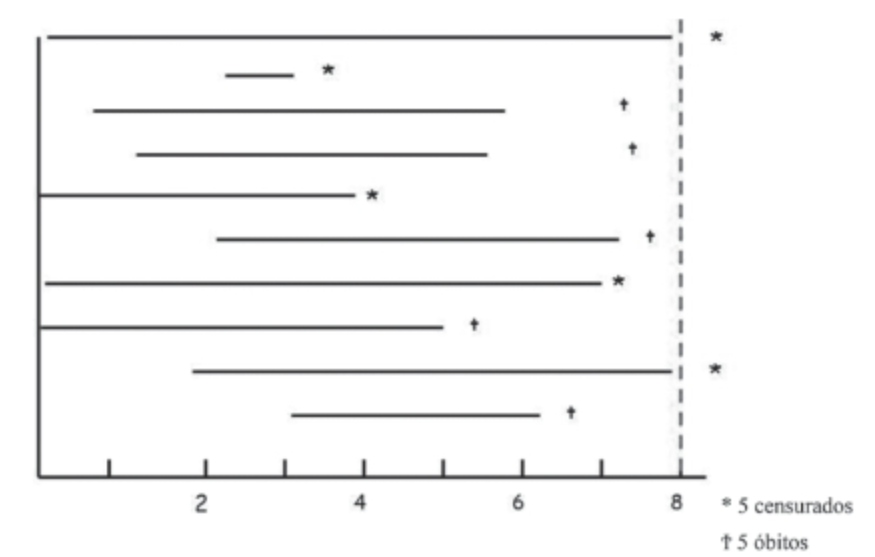
\includegraphics[width=6.25in,height=4.6875in]{../../images/censura.png}
\end{center}

\textbf{Dados censurados à direita:} maioria

\begin{center}
\pandocbounded{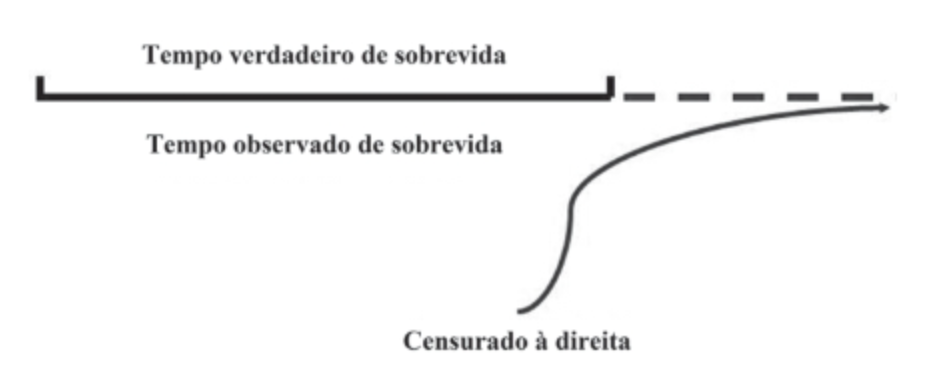
\includegraphics[keepaspectratio]{../../images/censura_direita.png}}
\end{center}

\subsection{Análise de
sobrevivência}\label{anuxe1lise-de-sobrevivuxeancia-2}

Indicada para estudos longitudinais (coorte, ensaios clínicos), ou seja,
o mesmo grupo de indivíduos é acompanhado durante um \textbf{intervalo
de tempo} preestabelecido pelo pesquisador.

. . .

A \textbf{grande vantagem} nesse tipo de análise é que se permite
utilizar informações de \textbf{todos} os participantes até o momento da
ocorrência do evento ou quando são censurados.

\subsection{Regressão de riscos}\label{regressuxe3o-de-riscos}

O modelo de sobrevida mais comum é o \textbf{modelo de riscos
proporcionais de Cox}. Este modelo permite que as covariáveis, numéricas
ou categóricas, variem com o tempo.

. . .

Assume-se, nesse modelo, que os tempos \(t_i\), \(i = 1, \cdots , n\),
são independentes e que a taxa de falha (risco) tem a seguinte forma:

\[\lambda(t) = \lambda_0(t) \exp (\beta_1 X_1 + \cdots + \beta_pX_p)\]

. . .

O componente não-paramétrico, \(\lambda_0(t)\), não é especificado e é
uma função não-negativa do tempo. Ele é usualmente chamado de função de
base ou risco basal.

\subsection{Regressão de riscos}\label{regressuxe3o-de-riscos-1}

O componente paramétrico \(\exp(\mathbf{x^t \beta})\) é o nosso
interesse, em especial no vetor de parâmetros \(\mathbf{\beta}\).

. . .

O modelo é conhecido por ter taxas de falhas proporcionais. Este fato é
conveniente na sua interpretação, ou seja, a razão das taxas de falha de
dois indivíduos diferentes \(i\) e \(j\) é dada por

\[\dfrac{\lambda_i(t)}{\lambda_j(t)} = \dfrac{\exp(\mathbf{x_i^t \beta})}{\exp(\mathbf{x_j^t \beta})} = \exp(\mathbf{x_i^t \beta} - \mathbf{x_j^t \beta}),\]
que não depende do tempo.

. . .

Assim, se um indivíduo no início do estudo tem um risco de morte igual a
duas vezes o risco de um segundo indivíduo, entao esta razão de riscos
será a mesma para todo o período de acompanhamento.

\subsection{Hazard Ratio (HR)}\label{hazard-ratio-hr}

O Hazard Ratio (HR) é uma medida estatística amplamente utilizada em
estudos de sobrevivência e análises de risco, especialmente em pesquisas
médicas e epidemiológicas.

. . .

Em um modelo de Cox, a razão de risco (HR) é usada para medir o efeito
de uma variável preditora no risco do evento.

. . .

É dada por

\[HR = \exp({\beta_i}), i = 1, \cdots, p,\] sendo \(\beta_i\) os
coeficientes estimados do modelo de regressão de cox.

\subsection{Hazard Ratio (HR)}\label{hazard-ratio-hr-1}

A HR representa o risco relativo do evento ocorrer para uma dada mudança
de unidade na variável preditora, com uma \(HR\) maior que 1 indicando
um risco aumentado e uma \(HR\) menor que 1 indicando um risco
diminuído.

\section{Exemplo}\label{exemplo-2}

\subsection{Descrição da base de
dados}\label{descriuxe7uxe3o-da-base-de-dados-4}

O conjunto de dados contém casos de um estudo que foi conduzido entre
1958 e 1970 no Hospital Billings da Universidade de Chicago sobre a
sobrevivência de pacientes que foram submetidos a cirurgia de mama. Os
dados incluem:

\begin{itemize}
\tightlist
\item
  Idade do paciente no momento da operação (numérico)
\item
  Ano da operação do paciente (ano - 1900, numérico)
\item
  Número de nódulos axilares positivos detectados (numérico)
\item
  Status de sobrevivência (dicotômica)

  \begin{itemize}
  \tightlist
  \item
    1 = o paciente sobreviveu 5 anos ou mais
  \item
    2 = o paciente morreu em 5 anos
  \end{itemize}
\end{itemize}

\subsection{Preparação}\label{preparauxe7uxe3o-2}

\subsubsection{Carregando os pacotes R}\label{carregando-os-pacotes-r-2}

\begin{Shaded}
\begin{Highlighting}[]
\NormalTok{pacman}\SpecialCharTok{::}\FunctionTok{p\_load}\NormalTok{(}
\NormalTok{  rio,}
\NormalTok{  tidyverse,}
\NormalTok{  survival,}
\NormalTok{  survminer}
\NormalTok{) }
\end{Highlighting}
\end{Shaded}

\subsection{Carregando os dados}\label{carregando-os-dados-2}

\begin{Shaded}
\begin{Highlighting}[]
\NormalTok{dados }\OtherTok{=}\NormalTok{ rio}\SpecialCharTok{::}\FunctionTok{import}\NormalTok{(}\StringTok{"https://raw.githubusercontent.com/tiagomartin/est104/refs/heads/master/dados/haberman.csv"}\NormalTok{)}

\NormalTok{dados }\SpecialCharTok{\%\textgreater{}\%} 
  \FunctionTok{str}\NormalTok{()}
\end{Highlighting}
\end{Shaded}

\begin{verbatim}
'data.frame':   306 obs. of  4 variables:
 $ idade  : int  30 30 30 31 31 33 33 34 34 34 ...
 $ anoOper: int  64 62 65 59 65 58 60 59 66 58 ...
 $ numNod : int  1 3 0 2 4 10 0 0 9 30 ...
 $ status : int  1 1 1 1 1 1 1 2 2 1 ...
\end{verbatim}

\subsection{Ajuste do modelo}\label{ajuste-do-modelo-2}

\begin{Shaded}
\begin{Highlighting}[]
\CommentTok{\# Ajustando o modelo de Cox}
\NormalTok{modelo\_cox }\OtherTok{\textless{}{-}} \FunctionTok{coxph}\NormalTok{(}\FunctionTok{Surv}\NormalTok{(idade, status}\SpecialCharTok{==}\StringTok{\textquotesingle{}2\textquotesingle{}}\NormalTok{) }\SpecialCharTok{\textasciitilde{}}\NormalTok{ ., }\AttributeTok{data =}\NormalTok{ dados)}

\CommentTok{\# Resumo do modelo}
\FunctionTok{summary}\NormalTok{(modelo\_cox)}
\end{Highlighting}
\end{Shaded}

\begin{verbatim}
Call:
coxph(formula = Surv(idade, status == "2") ~ ., data = dados)

  n= 306, number of events= 81 

            coef exp(coef) se(coef)      z Pr(>|z|)    
anoOper -0.02801   0.97238  0.03474 -0.806     0.42    
numNod   0.05517   1.05672  0.01009  5.469 4.52e-08 ***
---
Signif. codes:  0 '***' 0.001 '**' 0.01 '*' 0.05 '.' 0.1 ' ' 1

        exp(coef) exp(-coef) lower .95 upper .95
anoOper    0.9724     1.0284    0.9084     1.041
numNod     1.0567     0.9463    1.0360     1.078

Concordance= 0.631  (se = 0.041 )
Likelihood ratio test= 21.81  on 2 df,   p=2e-05
Wald test            = 30.08  on 2 df,   p=3e-07
Score (logrank) test = 32.88  on 2 df,   p=7e-08
\end{verbatim}

\subsection{Hazard Ratio (HR)}\label{hazard-ratio-hr-2}

\begin{Shaded}
\begin{Highlighting}[]
\FunctionTok{ggforest}\NormalTok{(modelo\_cox, }\AttributeTok{data =}\NormalTok{ dados)}
\end{Highlighting}
\end{Shaded}

\pandocbounded{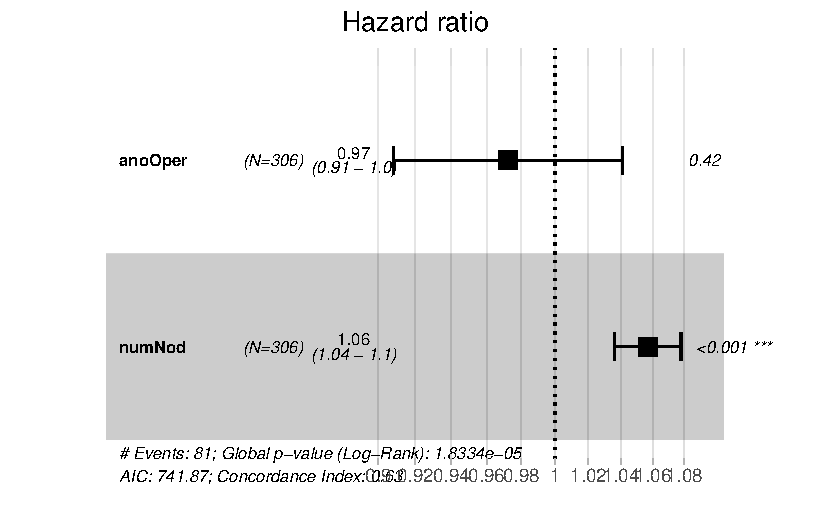
\includegraphics[keepaspectratio]{logistico_cox_files/figure-pdf/unnamed-chunk-13-1.pdf}}

\subsection{Interpretação}\label{interpretauxe7uxe3o}

O ano da operação do paciente não tem relação significativa com o
desfecho do paciente (\(p-valor = 0,42 > 0,05\)) ao nível de 5\% de
significância.

. . .

Já o número de nódulos axilares positivos detectados têm efeito
significativo na sobrevida dos pacientes. Cada aumento de um nódulo
detectado foi associado um aumento médio de 5,67\% no risco de
mortalidade do paciente em 5 anos, após considerar outras covariáveis.

. . .

O IC de 95\% para esse aumento ficou entre 3,6\% e 7,8\%
(\(p-valor << 0,001\))




\end{document}
